\documentclass{article}
\input{imports.tex}
\input{config.tex}

\begin{document}
\noindent \textbf{MA3701 Optimización}\\
\textbf{Profesor:} Alejandro Jofré\\
\textbf{Auxiliar:} Benjamín Vera Vera


\begin{center}
    \Huge{\textbf{Control 2}}\\
\textit{\large{Tiempo: 3:00}}\\
    \normalsize
    10 de noviembre de 2025
\end{center}

\begin{enumerate}
	\item Considere la función \(f : \mathbb{R}^n \to \mathbb{R}\) dada por \(f(x) = \norm{x}^3\). Se desea estudiar la convergencia del método de Newton con paso fijo \(\alpha > 0\) sobre esta función. Es decir, estudiamos iteraciones de la forma
		\[
			x_{k+1} = x_k - \alpha \qty(\nabla^2 f(x_k))^{-1} \nabla f(x_k).
		\]
		\begin{enumerate}
			\item (1 pt) Demuestre que para \(x \neq 0\),
				\[
					\nabla f(x) = 3 \norm{x} x, \qquad \nabla^2 f(x) = \frac{3}{\norm{x}} \qty(\norm{x}^2 I + xx^\top).
				\]
				\textbf{Solución:} Obtenemos primero el gradiente de \(g(x) = \norm{x}\). Para ello, vemos que
				\begin{align*}
					g(x) &= \sqrt{x_1^2 + \dots + x_n^2} \\
					\pdv{g}{x_i}(x) &= \frac{2x_i}{2 \sqrt{x_1^2 + \dots + x_n^2}} = \frac{x_i}{\norm{x}}.
				\end{align*}
				Entonces,
				\[
					\nabla g(x) = \frac{1}{\norm{x}} \mqty( x_1 \\ \vdots \\ x_n ) = \frac{x}{\norm{x}}.
				\]
				Ahora, usando la regla de la cadena, tenemos que
				\[
					\nabla f(x) = 3 \norm{x}^2 \cdot \nabla g(x) = 3 \norm{x}^2 \cdot \frac{x}{\norm{x}} = 3 \norm{x} x.
				\]
				\begin{center}
					\fbox{\textcolor{ForestGreen}{0.5pt.}}
				\end{center}
				Para el Hessiano, usamos la regla del producto, obteniendo que
				\begin{align*}
					\nabla^2 f(x) &= 3 \qty(\nabla(\norm{x}) x^\top + \norm{x} \nabla(x) ) \\
						      &= 3 \qty( \qty(\frac{x}{\norm{x}})x^\top + \norm{x}I ) \\
						      &= 3 \frac{xx^\top}{\norm{x}} + 3\norm{x}I \\
						      &= \frac{3}{\norm{x}} \qty(\norm{x}^2 I + xx^\top).
				\end{align*}
\begin{center}
					\fbox{\textcolor{ForestGreen}{0.5pt.}}
				\end{center}
			\item (2 pt) Calcule \((\nabla^2 f(x))^{-1}\). Para ello, puede utilizar la fórmula de inversión de Sherman-Morrison-Woodbury:
				\[
					\qty(A + ab^\top)^{-1} = A^{-1} - \frac{A^{-1} ab^\top A^{-1}}{1 + b^\top A^{-1}a}.
				\]
				\textbf{Solución:} Usando la parte anterior, tenemos que
				\begin{align*}
					(\nabla^2 f(x))^{-1} &= \frac{\norm{x}}{3} (\norm{x}^2 I + xx^\top)^{-1} \\
							     &= \frac{\norm{x}}{3} \qty( \frac{1}{\norm{x}^2}I - \frac{ \frac{1}{\norm{x}^2}I xx^\top \frac{1}{\norm{x}^2}I }{1 + x^\top \frac{1}{\norm{x}^2}I x} ) \\
							     &= \frac{\norm{x}}{3} \qty( \frac{1}{\norm{x}} I - \frac{\frac{1}{\norm{x}^4} xx^\top}{2} ) \\
							     &= \frac{1}{3\norm{x}} I - \frac{1}{6\norm{x}^3} xx^\top.
				\end{align*}
\begin{center}
					\fbox{\textcolor{ForestGreen}{1pt. Aplicar la fórmula, 1pt reducir. \textbf{Nota:} Puede que parte de esto ocurra en (c).}}
				\end{center}
			\item (2 pt) Concluya una fórmula general para la iteración del método de Newton \(x_{k+1}\) en términos de \(x_k\) y \(\alpha\).

				\textbf{Solución:} Reemplazando en la fórmula del método de Newton:
				\begin{align*}
					x_{k+1} &= x_k - \alpha \qty( \frac{1}{3\norm{x_k}}I - \frac{1}{6\norm{x_k}^3} x_k x_k^\top ) 3 \norm{x_k}x_k. \\
						&= x_k - \alpha \qty(x_k - \frac{1}{2} x_k) \\
						&= x_k - \alpha \frac{x_k}{2} \\
						&= \qty(1 - \frac{\alpha}{2})x_k.
				\end{align*}
\begin{center}
					\fbox{\textcolor{ForestGreen}{1pt. Utilizar correctamente la fórmula. 1pt reducir.}}
				\end{center}
			\item (1 pt) Encuentre el intervalo de valores \(\alpha > 0\) para que la sucesión generada por el método de Newton de paso \(\alpha\) sea convergente al mínimo global \(x^* = 0\) desde \textit{cualquier} punto inicial \(x_0 \in \mathbb{R}^n\).

				\textbf{Solución:} Ya que para esta función el método de Newton consiste en ponderar la iteración por un escalar, el método converge si dicho escalar es menor a 1 en módulo. Así, se requiere \(-1 < 1 - \frac{\alpha}{2} < 1 \iff \alpha \in (0, 4)\).
\begin{center}
					\fbox{\textcolor{ForestGreen}{1 pt. Obtener intervalo.}}
				\end{center}
		\end{enumerate}
	\item Sea \(f: \mathbb{R}^2 \to \mathbb{R}\) dada por
		\[
			f(x, y) = (x - 1)^2 + 4xy + y^4.
		\]
		\begin{enumerate}
			\item (2 pt) Encuentre todos los puntos críticos de \(f\) y decida cuáles de ellos son mínimos locales.

				\textit{Indicación} Pruebe que la matriz Hessiana \(\nabla^2 f(x, y)\) es semi-definida positiva si y solo si se tiene la condición
				\[
					3y^2 - 2 > 0.
				\]

				\textbf{Solución:} La condición de primer orden \(\nabla f(x, y)\) resulta en las ecuaciones
				\begin{align*}
					2(x-1) + 4y &= 0 \\
					x + y^3 &= 0.
				\end{align*}
				De la segunda, \(x = -y^3\), que reemplazando en la primera se reduce a
				\[
					y^3 - 2y + 1 = 0 \iff (y - 1)(y^2 + y + 1) = 0.
				\]
				Los puntos críticos son entonces dados por
				\[
					y = 1 , \frac{-1 \pm \sqrt{5}}{2}
				\]
\begin{center}
					\fbox{\textcolor{ForestGreen}{1 pt encontrar puntos críticos.}}
				\end{center}
				junto con sus correspondientes valores de \(x\) obtenidos por \(x = -y^3\). Para clasificar los puntos, vemos que el Hessiano de \(f\) es dado por
				\[
					\nabla^2 f (x, y) = \mqty(2 & 4 \\ 4 & 12y^2).
				\]
				La condición para que \(\lambda\) sea valor propio de esta matriz es la ecuación cuadrática
				\[
					\lambda^2 - (2 + 12y^2)\lambda + 24y^2 - 16 = 0.
				\]
				Se puede entonces usar la fórmula cuadrática para obtener la \textit{menor} solución a esta ecuación e imponer que sea estrictamente positiva. Esto se reduce a
				\[
					3y^2 - 2 > 0
				\]
\begin{center}
					\fbox{\textcolor{ForestGreen}{0.5 pt probar condición de segundo orden.}}
				\end{center}
				que es lo dado en la indicación. Esta condición la cumplen los puntos correspondientes a \(y = 1\) e \(y = \frac{-1 - \sqrt{5}}{2}\) junto con sus valores de \(x\) asociados. Así, los mínimos locales son:
				\begin{align*}
					(x_1, y_1) &= (-1, 1) \\
					(x_2, y_2) &= \qty(2 + \sqrt{5}, \frac{-1 - \sqrt{5}}{2}).
				\end{align*}
\begin{center}
					\fbox{\textcolor{ForestGreen}{0.5 pt aplicar y clasificar.}}
				\end{center}
			\item (2 pt) A partir de \(x_0 = (0, 2)\), efectúe dos iteraciones el método de gradiente con paso constante igual a \(1\). Entregue los puntos \(x_1, x_2\) correspondientes.

				\textbf{Solución:}
				\begin{align*}
					x_0 &= \mqty(0 \\ 2), \\
					x_1 &= \mqty(0 \\ 2) - \mqty(6 \\ 32) = \mqty(-6 \\ -30), \\
					x_2 &= \mqty(-6 \\ -30) - \mqty(-134 \\ -108.024) = \mqty(128 \\ 107.994).
				\end{align*}
\begin{center}
					\fbox{\textcolor{ForestGreen}{1pt obtener \(x_1\), 1pt obtener \(x_2\).}}
				\end{center}
			\item (1 pt) A partir de \(x_2\) la iteración obtenida en (b), efectúe una iteración del método de Newton con paso igual a \(1\). Entregue el punto \(x_3\) correspondiente.

				\textbf{Solución:} Aplicando la fórmula del método de Newton, se obtiene
				\[
					x_4 \approx \mqty(128 \\ 107.994) - \mqty(2 & 4 \\ 4 & 1,3\cdot10^{11})^{-1} \mqty(432.230 \\ 5,03\cdot10^{15}) \approx \mqty(-143.991 \\ 71.996).
				\]
\begin{center}
					\fbox{\textcolor{ForestGreen}{1pt. No se requiere exactitud numérica, pero sí deben corresponder las magnitudes y los signos.}}
				\end{center}
			\item (1 pt) ¿Qué está ocurriendo con las iteraciones? Discuta en relación a los mínimos obtenidos en (a).

				\textbf{Solución:} Claramente las iteraciones no están convergiendo a ninguno de los mínimos teóricos obtenidos. Esto parece deberse a que los pasos en ambos métodos son demasiado extensos. Debería realizarse búsqueda de línea para obtener una búsqueda más precisa.
\begin{center}
					\fbox{\textcolor{ForestGreen}{1pt. Debe haber discusión sobre el paso, aunque no necesariamente proponer una solución.}}
				\end{center}
		\end{enumerate}
	\item Considere el problema con restricciones siguiente:
		\begin{align*}
			(\text{P}) : \min_{x_1, x_2}\; & x_1 + 2x_2 \\
					& \frac{1}{4} x_1^2 + x_2^2 - 1 = 0.
		\end{align*}
		\begin{enumerate}
			\item (1 pt) Utilizando las condiciones de KKT, encuentre todos los puntos críticos de este problema.
				\textbf{Solución:} Consideramos el Lagrangeano del problema \(L(x_1, x_2, \mu) = (x_1 + 2x_2) + \mu\qty( \frac{1}{4} x_1^2 + x_2^2 - 1)\). Con esto, tenemos las condiciones:
				\begin{align}
					1 + \frac{\mu x_1}{2} &= 0, \label{KKT-1} \\
					2 + 2 \mu x_2 & = 0, \label{KKT-2} \\
					\frac{1}{4} x_1^2 + x_2^2 - 1 &= 0. \label{PF}
				\end{align}
				\begin{center}
					\fbox{\textcolor{ForestGreen}{0.5pt. Obtener condiciones.}}
				\end{center}
				Vemos que las condiciones \eqref{KKT-1}, \eqref{KKT-2} no se pueden cumplir si \(\mu = 0\), por lo que podemos suponer \(\mu \neq 0\) y despejar obteniendo
				\begin{align*}
					x_1 & = -\frac{2}{\mu}, \\
					x_2 &= -\frac{1}{\mu}.
				\end{align*}
				Reemplazando en \eqref{PF}, tenemos que \(\mu = \pm \sqrt{2}\). De modo que se obtienen los puntos críticos:
				\begin{align*}
					(x_1, x_2) &= \qty( -\sqrt{2}, -\frac{\sqrt{2}}{2} ), \\
					(x_1, x_2) &= \qty(\sqrt{2}, \frac{\sqrt{2}}{2}).
				\end{align*}
				\begin{center}
					\fbox{\textcolor{ForestGreen}{0.5pt. Resolver.}}
				\end{center}

			\item (1 pt) Esboce el conjunto factible de este problema así como el gradiente de la función objetivo. Utilice esto para decidir cuál de los puntos críticos obtenidos es mínimo del problema.

				\textbf{Solución:} El gradiente de la función objetivo, es el vector \((1, 2)\). Además, el conjunto factible corresponde a una elipse centrada en \((0, 0)\) en la siguiente forma:

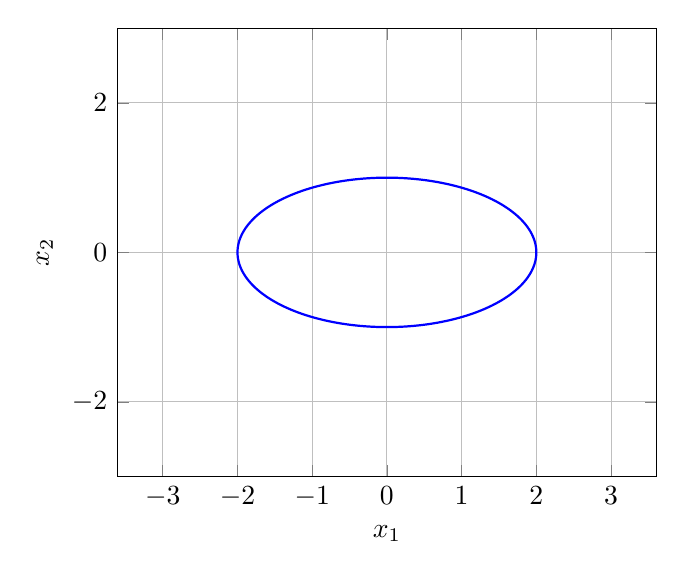
\begin{tikzpicture}
  \begin{axis}[
    axis equal,
    xlabel={$x_1$},
    ylabel={$x_2$},
    grid=both,
    xmin=-3, xmax=3,
    ymin=-3, ymax=3,
    samples=200,
  ]

    % Ellipse: (1/4)x1^2 + x2^2 = 1
    \addplot[
      domain=0:360,
      smooth,
      thick,
      blue
    ] ({2*cos(x)}, {sin(x)});
  \end{axis}
\end{tikzpicture}

Con esto, podemos deducir que el mínimo real de la función corresponde al punto \((x_1, x_2) = \qty( -\sqrt{2}, -\frac{\sqrt{2}}{2} )\). El otro punto es en realidad un máximo.
				\begin{center}
					\fbox{\textcolor{ForestGreen}{1pt. Argumentar.}}

						\textcolor{ForestGreen}{\textbf{Nota:} Mientras el argumento sea válido, el desarrollo es correcto aún si no se construye el gráfico pedido.}
				\end{center}

			\item (2 pt) Dado \(\epsilon>0\), considere el método de penalización cuadrática, con el cual se obtiene el problema irrestricto
				\[
					(\text{P}_{\epsilon}) : \min_{x_1, x_2 \in \mathbb{R}} f_\epsilon(x_1, x_2) := (x_1 + 2x_2) + \frac{1}{2\epsilon} \qty(\frac{1}{4} x_1^2 + x_2^2 - 1)^2.
				\]
				Obtenga condiciones que describan los puntos críticos de \(f_\epsilon\).

				\textbf{Solución:} La condición de primer orden es dada por:
				\begin{align}
					1 + \frac{1}{\epsilon}\qty( \frac{1}{4}x_1^2 + x_2^2 - 1 ) \frac{x_1}{2} &= 0, \label{CP1} \\
					2 + \frac{1}{\epsilon}\qty(\frac{1}{4}x_1^2 + x_2^2 - 1) 2x_2 &= 0. \label{CP2}
				\end{align}
				\begin{center}
					\fbox{\textcolor{ForestGreen}{1pt. Obtener condiciones}}
				\end{center}

				Multiplicando \eqref{CP1} por \(2\) y restando, se obtiene entonces que
				\[
					\qty(\frac{1}{4} x_1^2 + x_2^2 - 1)(x_1 - 2x_2) = 0.
				\]
				El primer término no puede ser \(0\) debido a las ecuaciones \eqref{CP1} y \eqref{CP2}. Por lo que necesariamente se tiene
				\[
					x_1 = 2x_2.
				\]
				Reemplazando esto en \eqref{CP1}, se obtiene que
				\[
					2x_2^3 - x_2 + \epsilon = 0.
				\]
				Entonces, la condición de optimalidad es que \(x_1 = 2x_2\) con \(x_2\) raíz de la función cúbica:
				\[
					g(x) = 2x^3 - x + \epsilon.
				\]
				\begin{center}
					\fbox{\textcolor{ForestGreen}{1pt. Simplificar y describir.}}
				\end{center}

			\item (2 pt) Haciendo uso de las condiciones obtenidas en (c), encuentre una cota inferior sobre \(\epsilon\) para que exista un solo punto crítico. Describa lo que podría ocurrir con el algoritmo de penalización si esta condición no se cumple.

				\textbf{Solución:} En vista de lo anterior, nos basta analizar la existencia de una sola raíz de la función \(g\). Para esto, obtenemos los puntos críticos de \(g\):
				\[
					g'(x) = 6x^2 - 1 = 0 \implies x = \pm \frac{1}{\sqrt{6}}.
				\]
				Ya que \(g''(x) = 12x\), el mínimo es dado por \(x^* = \frac{1}{\sqrt{6}}\). El \textit{valor} mínimo local de la función \(g\) es entonces
				\[
					g\qty( \frac{1}{\sqrt{6}} ) = 2 \qty(\frac{1}{\sqrt{6}})^3 - \frac{1}{\sqrt{6}} + \epsilon.
				\]
				Así, si este mínimo es positivo, tenemos una única raíz de la cúbica y por lo tanto un único punto crítico de la función \(f_\epsilon\). La condición es entonces
				\[
					\epsilon > \frac{1}{\sqrt{6}} - \frac{2}{\sqrt{6^3}} \approx 0.27.
				\]
				\begin{center}
					\fbox{\textcolor{ForestGreen}{1pt. Obtener cota.}}
				\end{center}
				Si esta cota inferior no se cumpliera, entonces un algoritmo de minimización para la función \(f_\epsilon\) podría converger a puntos ficticios que no tienen relación con el mínimo conocido del problema original. Así, una penalización de restricciones demasiado exigente puede resultar en mal condicionamiento del problema.
				\begin{center}
					\fbox{\textcolor{ForestGreen}{1pt. Discusión.}}
				\end{center}

		\end{enumerate}
\end{enumerate}

\end{document}
